\documentclass[conference]{IEEEtran}
\IEEEoverridecommandlockouts

\usepackage{cite}
\usepackage{graphicx}
\usepackage{url}
\usepackage{hyperref}
\usepackage{amsmath}
\usepackage{amssymb}
\usepackage{tikz}

\title{
Automated Post-Incident Policy Gap Analysis via Threat-Informed Evidence Mapping using Large Language Models
}

\author{
\IEEEauthorblockN{Oh Huan Lin, Jay Yong Jun Jie, Lee Ling Siu Mandy, Dr Jonathan Pan}
\IEEEauthorblockA{
Nanyang Technological University, Singapore \\
Emails: W240001@e.ntu.edu.sg, JAYY0002@e.ntu.edu.sg, MANDY001@e.ntu.edu.sg, 
JonathanPan@ntu.edu.sg 
}
}

\begin{document}
\maketitle

\begin{abstract}
Cybersecurity post-incident reviews are essential for identifying control failures and improving organisational resilience, yet they remain labour-intensive, time-consuming, and heavily reliant on expert judgment. This paper investigates whether Large Language Models (LLMs) can augment post-incident review workflows by analysing system evidence and identifying candidate security policy gaps. We present a threat-informed, agentic framework that ingests log data, maps observed behaviours to the MITRE ATT\&CK framework, and evaluates organisational security policies for adequacy and compliance. Using a simulated brute-force attack scenario against a Windows OpenSSH service (MITRE ATT\&CK T1110), the system leverages GPT-4o for reasoning, LangGraph for workflow orchestration, and policy-snippet retrieval for traceable policy comparison. Experimental results indicate that the LLM-based pipeline can interpret log-derived evidence, identify insufficient or missing policy controls, and generate actionable remediation recommendations with explicit evidence-to-policy traceability. Unlike prior work that treats log analysis and policy validation as isolated tasks, this study integrates both into a unified end-to-end proof-of-concept post-incident review framework. The findings suggest that LLM-assisted analysis has the potential to improve the efficiency, consistency, and auditability of post-incident evaluations, while highlighting the continued need for human oversight in high-stakes cybersecurity decision-making.
\end{abstract}
\begin{IEEEkeywords}
Large Language Models, Agentic AI, Cybersecurity, Post-Incident Review, Policy Compliance, MITRE ATT\&CK
\end{IEEEkeywords}

\section{Introduction}
Cybersecurity post-incident reviews are essential for identifying control failures, understanding attacker behaviour, and improving organisational security posture \cite{Connolly2025PostIncident, AtlassianPostmortem}. In practice, these reviews remain largely manual and expert-driven, particularly when correlating large volumes of system logs with organisational security policies \cite{Antunes2022Audit, Hanson2021ICS}. As cyber threats evolve rapidly, static and infrequently reviewed policies increasingly struggle to reflect real-world attack techniques and operational conditions \cite{Linkov2014Risk, Hill2021Bruteforce}.

Recent advances in Large Language Models (LLMs) suggest potential for post-incident analysis workflows that require reasoning over semi-structured evidence \cite{Huang2023ReasoningSurvey, Wei2022CoT}. However, prior work has mostly examined isolated tasks such as log analysis or policy compliance checking rather than integrated workflows that connect technical evidence to governance-oriented policy evaluation \cite{Zhang2025Survey, Cadet2024Compliance}. 

This paper evaluates whether an LLM-driven workflow can support post-incident reviews by analysing log-derived evidence, mapping observed behaviour to MITRE ATT\&CK, and identifying policy gaps in a traceable manner. In contrast to document-centric compliance agents that begin from policy texts and standards, the proposed workflow begins from incident evidence and asks whether documented controls were adequate under the observed attack conditions. The goal is not analyst replacement, but feasibility-focused decision support.

The contributions of this paper are as follows:
\begin{itemize}
    \item An end-to-end, agentic post-incident review workflow integrating log analysis, threat attribution, and policy gap identification.
    \item A threat-informed evidence-to-policy mapping approach grounded in the MITRE ATT\&CK framework.
    \item An interpretable and auditable workflow design to support governance and compliance-oriented post-incident evaluation.
\end{itemize}


\section{Related Work}

Recent studies show that LLMs can assist with log interpretation, vulnerability analysis, and partial audit automation \cite{Chin2025Audit, Ruan2023Agents, Fang2024Hack}. Agentic systems have also supported SOC orchestration, incident handling, and MITRE ATT\&CK mapping \cite{Jin2024Crimson, Licitra2024SOCAI}. In parallel, LLM-based audit and compliance work has focused on interpreting regulatory text and comparing documented controls \cite{Cadet2024Compliance, Salman2024Compliance}. Recent work such as MACAW further demonstrates that agentic AI can automate policy-to-standard compliance analysis against frameworks such as NIST 800-53 and ISO 27002 with strong agreement against expert decisions \cite{Negi2026MACAW}. Traditional audits and postmortems, however, remain largely manual and policy-centric \cite{Antunes2022Audit, AtlassianPostmortem}. 

The gap is that these strands are rarely combined into a single post-incident workflow that connects log-derived evidence, threat abstraction, and organisational policy evaluation with explicit traceability. Prior SOC and SIEM-oriented systems generally emphasise triage, alert enrichment, or response coordination, while compliance-oriented systems usually begin from policy text and compare controls in a document-centric manner. Unlike those approaches, the proposed workflow starts from incident evidence and ends with policy-gap findings, line-window policy support, and remediation suggestions. This study addresses that gap in a scoped scenario: a simulated Windows OpenSSH brute-force incident mapped to MITRE ATT\&CK T1110, using EVTX-derived CSV data and organisational account-management policies.


\section{Methodology}

\subsection{Agentic Workflow Architecture}
The system is implemented as a multi-agent, shared-state pipeline orchestrated with LangGraph \cite{LangGraph2025, Taulli2025LangGraph}. Agents perform log interpretation, threat attribution, policy retrieval, policy comparison, evidence validation, and report generation while reading from and writing to a shared global state. GPT-4o is used for reasoning, and the retrieval layer preserves approximate line-window metadata for policy comparison. This architecture supports traceable information flow across stages and allows intermediate outputs to be reused and validated.

\subsection{Incident Data and Threat Attribution}
The experiment uses Windows Event Log (EVTX) data representing a brute-force attack against a Windows OpenSSH service. EVTX files are deterministically converted to XML and then flattened to CSV before being supplied to the workflow. The log analysis agent examines authentication-related events and maps the observed behaviour to MITRE ATT\&CK T1110 (Brute Force), providing a standard threat context for downstream policy evaluation \cite{MITREATTACK}. The selected dataset contains successful OpenSSH-related logon activity and a later burst of repeated authentication failures, making it suitable for evaluating both threat attribution and access-control policy adequacy.


\subsection{Policy Evaluation and Evidence Traceability}
Organisational policies and baseline controls are ingested as PDFs and converted into line-window snippets for comparison. When vector indexing is enabled, LlamaIndex is used for semantic retrieval; otherwise, the implementation falls back to deterministic keyword-based snippet retrieval. Relevant clauses are compared against the organisation's policy and converted into candidate gaps with supporting log evidence, policy excerpts, and qualitative confidence labels. The implemented baseline corpus uses CIS Controls excerpts as the comparison baseline, while broader governance references such as NIST SP 800-53 and ISO/IEC 27001 provide contextual grounding for the audit domain \cite{NIST80053,ISO27001,CISControls}.


\subsection{Implementation Details and Prompt Control}
Preprocessing is deterministic and performed outside the LLM: EVTX logs are converted to XML and flattened to CSV before analysis. Prompts are role-specific and constrained to observable evidence and retrieved policy text. For example, the evidence-analysis prompt asks for a summary grounded in concrete log fields, while the policy-comparison prompt requires JSON-formatted gaps using only the supplied policy snippets and line-window references.

A representative evidence-analysis prompt template is: ``You are a cyber analyst. Summarize indicators from the Windows/OpenSSH logs. Focus on event IDs, timestamps, source IPs, target accounts, failure counts, lockouts, and brute-force indicators. Support the summary with specific rows and fields you see.'' A representative policy-comparison prompt template is: ``You are an auditor. Compare Baseline (Policy A) versus Target (Policy B). Use only the provided policy snippets; do not invent citations. Return JSON list of gaps with gap title, rationale, remediation, and line-window references copied verbatim from the supplied snippets.'' In both cases, the grounding constraint is explicit: evidence summaries must remain tied to observable log fields, and policy-gap generation must remain tied to retrieved policy excerpts.

For reproducibility, the implementation uses OpenAI model aliases rather than a pinned snapshot: GPT-4o is used for evidence analysis, policy comparison, evidence validation, and report generation; it is also used for policy selection when policy documents are not preselected by the runner. Optional LlamaIndex policy-index construction uses the OpenAI \texttt{text-embedding-3-small} embedding model. All inference nodes use temperature 0. The LangGraph workflow contains ten executable nodes grouped into the six roles shown in Figure~\ref{fig:workflow}; the shared state stores the threat description, log path and loaded data, evidence summary, evidence-derived control expectations, selected policies, retrieved snippets, gap objects, evidence mappings, and final report. Retrieval uses LlamaIndex with similarity\_top\_k=10 when vector indexes are enabled and keyword snippet retrieval otherwise. The primary policy corpus contains two PDFs totalling four pages, and the primary log dataset contains one CSV with 11 event rows. Confidence is a qualitative low/medium/high label produced by the evidence-validation agent rather than a calibrated score.

\begin{figure}[h]
\centering
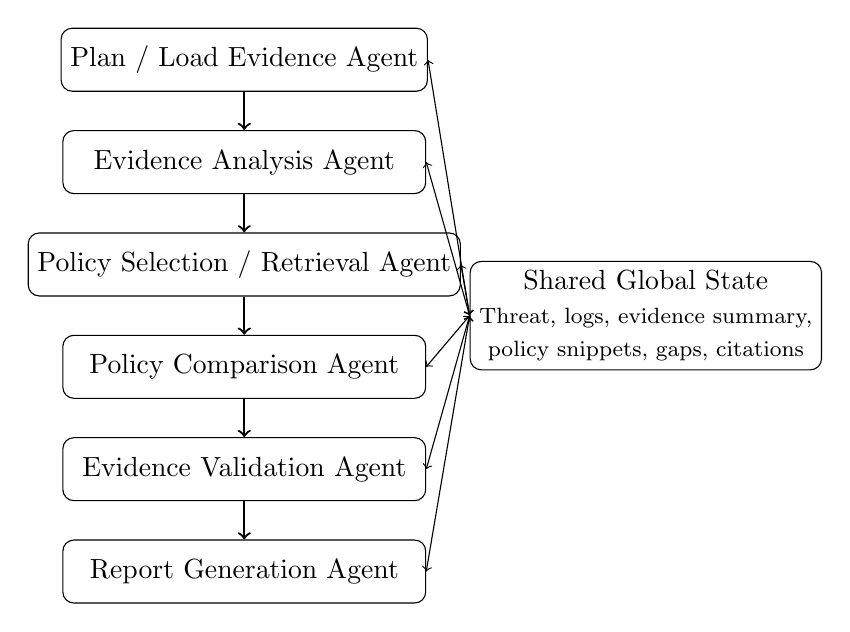
\begin{tikzpicture}[
    agent/.style={
        draw,
        rounded corners,
        align=center,
        minimum width=0.38\linewidth,
        minimum height=0.8cm
    },
    statebox/.style={
        draw,
        rounded corners,
        align=center,
        minimum width=0.34\linewidth,
        minimum height=1.1cm
    },
    arrow/.style={->, thick},
    statearrow/.style={<->, thin}
]

\node[agent] (plan) at (0,0) {Plan / Load Evidence Agent};
\node[agent] (analyze) at (0,-1.3) {Evidence Analysis Agent};
\node[agent] (retrieve) at (0,-2.6) {Policy Selection / Retrieval Agent};
\node[agent] (compare) at (0,-3.9) {Policy Comparison Agent};
\node[agent] (validate) at (0,-5.2) {Evidence Validation Agent};
\node[agent] (report) at (0,-6.5) {Report Generation Agent};

\node[statebox] (state) at (5.1,-3.25) {Shared Global State\\
\footnotesize Threat, logs, evidence summary,\\
\footnotesize policy snippets, gaps, citations};

\draw[arrow] (plan) -- (analyze);
\draw[arrow] (analyze) -- (retrieve);
\draw[arrow] (retrieve) -- (compare);
\draw[arrow] (compare) -- (validate);
\draw[arrow] (validate) -- (report);

\draw[statearrow] (plan.east) -- (state.west);
\draw[statearrow] (analyze.east) -- (state.west);
\draw[statearrow] (retrieve.east) -- (state.west);
\draw[statearrow] (compare.east) -- (state.west);
\draw[statearrow] (validate.east) -- (state.west);
\draw[statearrow] (report.east) -- (state.west);

\end{tikzpicture}
\caption{Sequentially orchestrated multi-agent workflow with shared global state}
\label{fig:workflow}
\end{figure}



\section{Findings}

\begin{table*}[t]
\centering
\caption{Example end-to-end output from the implemented workflow}
\scriptsize
\setlength{\tabcolsep}{2pt}
\begin{tabular}{|p{0.15\textwidth}|p{0.11\textwidth}|p{0.17\textwidth}|p{0.16\textwidth}|p{0.17\textwidth}|p{0.06\textwidth}|}
\hline
\textbf{Log evidence} & \textbf{Threat mapping} & \textbf{Retrieved policy evidence} & \textbf{Identified gap} & \textbf{Recommendation} & \textbf{Conf.} \\
\hline
Five Event ID 4625 failed logon events for \texttt{admmig@offsec.lan} occurred between 20:43:22 and 20:43:50, with OpenSSH-related authentication activity and earlier Event ID 4624 successful logon events also present in the dataset. &
MITRE ATT\&CK T1110: Brute Force. &
The system retrieved APN User Account Policy line-window evidence covering the account-lockout clause and CIS account-management snippets for contextual comparison. &
Account lockout threshold gap: the target policy specifies lockout after 12 consecutive failed attempts, which may be too lenient under the observed brute-force pattern. &
Review and tune the target policy's lockout threshold, and improve logging or monitoring for repeated failed OpenSSH authentication attempts. &
Medium \\
\hline
\end{tabular}
\label{tab:end_to_end_output}
\end{table*}

\begin{table}[t]
\centering
\caption{Consistency across repeated executions of the same scenario ($N=5$)}
\scriptsize
\setlength{\tabcolsep}{3pt}
\begin{tabular}{|p{0.34\columnwidth}|p{0.22\columnwidth}|p{0.31\columnwidth}|}
\hline
\textbf{Metric} & \textbf{Result} & \textbf{Observation} \\
\hline
Successful executions & 5/5 & All repeated runs completed and produced a report. \\
\hline
Brute-force interpretation & 5/5 & All runs described the Event ID 4625 burst as brute-force activity. \\
\hline
Account lockout threshold gap & 5/5 & This was the stable incident-relevant finding across all repeated runs. \\
\hline
APN lockout-policy citation returned & 5/5 & Every run linked the finding to the APN account-lockout line-window. \\
\hline
Additional MFA gap & 1/5 & One run surfaced an additional MFA-related finding, indicating some residual variation. \\
\hline
Unsupported password-age or complexity gaps & 0/5 & Evidence-gating removed the earlier unsupported password-policy findings. \\
\hline
\end{tabular}
\label{tab:consistency_results}
\end{table}

\begin{table}[t]
\centering
\caption{Illustrative baseline comparison for the same scenario}
\scriptsize
\setlength{\tabcolsep}{3pt}
\begin{tabular}{|p{0.24\columnwidth}|p{0.14\columnwidth}|p{0.22\columnwidth}|p{0.20\columnwidth}|}
\hline
\textbf{Method} & \textbf{Time} & \textbf{Evidence handling} & \textbf{Output} \\
\hline
Illustrative manual review & Approx. 18 min & Human review of the same logs and policy documents. & Manual threat interpretation, policy comparison, and recommendations. \\
\hline
Full LLM workflow & End-to-end runner mean 37.4 s (32.9--42.6 s) & Interpreted the log pattern, retrieved policy text, and preserved line-window citations. & Produced policy-gap findings, evidence linkage, and recommendations. \\
\hline
\end{tabular}
\label{tab:baseline_comparison}
\end{table}

Across five repeated executions, the workflow repeatedly interpreted the authentication burst as brute-force behaviour and returned line-window policy evidence in every run (Table~\ref{tab:consistency_results}). The stable incident-relevant finding was the account lockout threshold gap, which appeared in all five runs and was consistently linked to the APN policy line-window containing the 12-failed-attempt lockout clause. The evidence-validation stage labelled this finding as indirectly supported by the logs: the logs directly show repeated Event ID 4625 failures, while the policy conclusion concerns whether the documented threshold is sufficiently strict under that observed attack pattern. One run also surfaced an MFA-related finding, indicating some residual variation, but unsupported password-age and password-complexity gaps did not recur after evidence-gating was added. In the representative output in Table~\ref{tab:end_to_end_output}, the system mapped the event pattern to MITRE ATT\&CK T1110 and linked the lockout-threshold finding to explicit log indicators and target-policy line ranges. A second repeated-run check on the supplementary PowerShell HTTP-listener case also completed successfully in all five runs. It consistently recovered network monitoring and alerting gaps, while retention-of-monitoring-records appeared in all five runs and PowerShell logging or listener-approval findings appeared in subsets of the runs.

Operationally, the primary brute-force workflow completed in an end-to-end runner mean of 37.4 seconds across five runs, compared with an illustrative manual review time of approximately 18 minutes (Table~\ref{tab:baseline_comparison}). The supplementary PowerShell workflow completed in an end-to-end runner mean of 50.8 seconds across five runs. These timings are machine-, network-, and API-dependent, but they show that the pipeline can produce integrated gap findings, evidence linkage, and recommendations rather than only a threat label. Explicit log references, retrieved snippets, and line-window citations help constrain unsupported claims, but they do not eliminate hallucination risk; human review remains necessary before audit or operational use.

As a compact second example, the workflow was also examined against a public Windows telemetry trace labelled as a PowerShell HTTP Listener scenario \cite{Rodriguez2020PowerShellHTTPListener}. In that trace, repeated PowerShell-related Sysmon events appeared on host \texttt{WORKSTATION5}, and Windows Filtering Platform events recorded a local listener on TCP port 8000. The evidence was sufficient for a qualitative threat interpretation consistent with suspicious PowerShell-based execution and exposed listening behaviour, although the dataset did not include command-line fields or full parent-child process context. This supplementary case therefore supports breadth across a second ATT\&CK-relevant behaviour family, while remaining weaker than the primary brute-force case for detailed evidence-to-policy comparison. Taken together, the two cases suggest that the same multi-agent workflow can be reused across multiple incident patterns, provided that the available logs still expose enough evidence for grounded interpretation and policy retrieval.


\section{Discussion}
The study suggests that LLMs can augment post-incident reviews by linking technical evidence and policy evaluation within a single traceable process. The main benefit is not autonomous decision-making, but structured decision support: the workflow can summarise evidence, retrieve relevant policy text, and surface candidate gaps with explicit citations. This is particularly useful in governance-oriented settings where analysts need not only an incident interpretation, but also a defensible explanation of why an existing policy may be insufficient under observed attack conditions.

The repeated-run results also show the current boundary of reliability. Threat interpretation and citation grounding were stable, whereas gap prioritisation still varied. In practice, this means the workflow is better suited to accelerating analyst review and narrowing attention to plausible control weaknesses than to making fully autonomous compliance judgments. The strongest value of the approach is therefore in reducing the effort required to move from raw incident evidence to a first-pass, policy-aware assessment that a human analyst can then verify and refine.

This positioning also helps frame the contribution more realistically. The work does not claim state-of-the-art attack detection or general compliance automation. Instead, it demonstrates that an LLM-based workflow can bridge a gap that is often left manual: translating incident evidence into governance-relevant findings with explicit traceability. Accordingly, the system is best viewed as a governance-oriented analyst aid whose outputs require human confirmation before audit or operational use.


\section{Limitations}
The evaluation is centred on one fully developed brute-force scenario over Windows Event Logs, with only a compact supplementary PowerShell listener example, so the findings may not transfer directly to multi-stage attacks, cloud telemetry, endpoint traces, or other heterogeneous evidence sources. The workflow also relies on a single reasoning model, and repeated runs show that some variability remains despite temperature control and structured prompts. As a result, the current study cannot establish generalisability across attack classes, organisations, or model families.

Policy-gap quality also depends on the completeness, specificity, and writing quality of the source documents. Ambiguous or weakly documented policies may reduce retrieval precision or lead to under-specified findings even when the threat interpretation is correct. The supplementary PowerShell trace further illustrates that public datasets may expose timestamps, hostnames, and process images while omitting command-line content or richer user context, which limits the granularity of downstream policy assessment. In addition, the study focuses on feasibility rather than large-scale benchmarking, so it does not report expert agreement, precision/recall-style metrics, or systematic comparisons against non-agentic baselines. Any operational deployment would also need to address data governance, privacy, access control, and accountability when handling sensitive logs and policies through external APIs.

\section{Future Work}
Future work should evaluate the workflow on additional scenarios beyond brute-force authentication, including privilege escalation, lateral movement, malware execution, and suspicious PowerShell activity. It would also be valuable to compare the current multi-agent design against simpler baselines such as single-prompt LLM analysis, non-agentic retrieval-augmented generation, and analyst-only review. Broader validation should include expert-assessed gap quality, agreement across repeated runs, and operational studies on privacy, access control, and secure enterprise deployment.

\section{Conclusion}
This paper evaluated a feasibility-focused LLM-assisted workflow for post-incident policy gap analysis. By integrating log analysis, threat attribution, policy retrieval, and evidence-linked gap identification, the workflow demonstrates how incident evidence can be connected to governance review in a traceable manner. Unlike document-centric compliance agents, the proposed approach begins from observed incident evidence and evaluates whether documented controls were adequate under the attack conditions. The results suggest practical value for decision support, while also showing that human oversight remains necessary because gap prioritisation still varies across runs.

\section{Code availability}
The GitHub repository will be made publicly available after acceptance of the paper.


\bibliographystyle{IEEEtran}
\bibliography{references}

\end{document}
